\subsection{Diagramme de séquence}
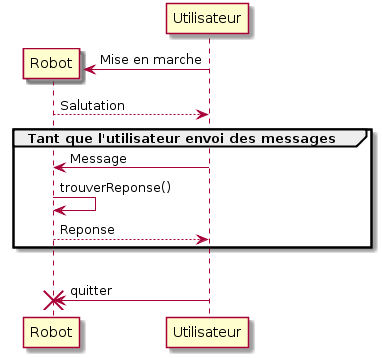
\includegraphics[scale=0.5]{diagrammedeSequence.png}
\subsection{Représentation de l'information}
\subsubsection{Mot}
Le mot est l'unité atomique de la phrase. Il est représenté par une chaine de caractère sans espace. En français, le radical est la plupart du temps constant dans les mots d'une même famille. Ainsi, il n'est pas nécessaire de changer le radical, mais simplement la terminaison du mot, d'où la nécessité de pouvoir influer sur les quelques dernières lettres en ajoutant ou supprimant celles-ci.
\subsubsection{Phrase}
La phrase est un ensemble de mot, visant à exprimer des concepts. Elle contiendra donc un tableau de mot de longueur indéterminée. A cela s'ajoute la ponctuation finale qui spécifie si la phrase est interrogative ou affirmative. Cette ponctuation finale sera donc aussi stockée en mémoire dans un caractère dédié. Le sens d'une phrase étant défini par certains mots tels que pronoms et verbes, savoir si un mot en particulier est présent dans la phrase.
Enfin, afin de créer une réponse sensée, il est nécessaire de pouvoir créer une phrase en s'appuyant sur les mots de la phrase précédente.
\subsubsection{Robot}
En français, la position de chaque mot est importante car elle a une influence sur la phrase. La grammaire française est une grammaire complexe. Cependant, contrairement à l'allemand, la position des mots n'est pas absolument figée, et grâce au virgules notamment, il est possible de séparer le sujet de son verbe. Le succès des robots dans ce domaine reste encore très limité, et faute de temps et de moyens, nous nous limiterons au traitement de phrase simple, avec un sujet précédant directement son verbe.

\begin{figure}
    \center
	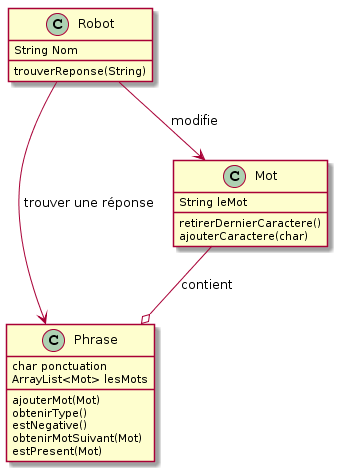
\includegraphics[scale=0.5]{diagrammeDeClasse.png}
	\caption{Diagramme de classe}
\end{figure}
